\section{\label{II-B-3}Les ontologies dans le Web sémantique}
\titreEntete{Les ontologies dans le Web sémantique}

%intro
La finalité principale des ontologies est leur exposition sur le Web de données. L'utilisation qui s'ensuit permet la création d'un Web sémantique, structuré avec des données partagées. Le référentiel compris dans le sens de \ac{kos} n'est plus aussi présent dans ce Web sémantique; le modèle de description de ces référentiels s'impose sous la forme des ontologies et améliore dans le même temps, par des relations typées, la description des concepts qu'il contient.\\

Cette avancée permet une description plus fine et partagée des documents des institutions patrimoniales: le référentiel est à la fois leurs propres données et celles du Web de données, liées par les ontologies publiques.

\subsection{\label{II-B-3-a}Décrire des ontologies en \ac{rdf}: \ac{rdfs} et \ac{owl}}
\titreEntete{Décrire des ontologies en RDF}

De même que \ac{skos} est une ontologie permettant la description de \ac{kos}, \index[ref]{relier@Relier!rdfs@RDFS}\ac{rdfs} et \index[ref]{relier@Relier!owl@OWL}\ac{owl} sont les représentations des ontologies \index[ref]{echanges@Échanges!formats@Formats!rdf@RDF}\ac{rdf}. Les documents décrits par les institutions le sont par des formats et des logiques différentes. Utiliser une seule ontologie peut s'avérer difficile; en effet, elle peut être trop large ou trop spécifique pour le domaine décrit. C'est pourquoi l'utilisation des URIs, des liens hypertexte du Web, permet d'utiliser autant d'ontologies que nécessaire, et de créer une interopérabilité par parcours de liens, par rebonds sur les URIs.\\

La constitution de ce réseau de liens, utilisé pour la description de documents, n'est possible qu'avec l'utilisation du \index[ref]{typologie@Typologie!graphe@Graphe de nœuds et de liens}Web sémantique et de \index[ref]{echanges@Échanges!formats@Formats!rdf@RDF}\ac{rdf}. C'est pourquoi il a été nécessaire de construire des modèles de représentation des ontologies en \ac{rdf}.\\

\ac{rdfs} est un langage de description simple, destiné à apporter les bases d'une description en \ac{rdf} avec la déclaration de classes --- et de sous-classes --- et de propriétés. Les classes sont des concepts, des types de ressources, identifiés par des URIs. Les propriétés sont les relations qui existent entre les classes. Ainsi, chaque ressource est instanciée à une classe par la propriété --- le prédicat \ac{rdf} --- <http://www.w3.org/1999/02/22-rdf-syntax-ns\#type> (rdf:type). La présence de sous-classes permet de créer des groupes au sein de classes: en déclarant une instance d'une sous-classe, un second triplet est alors implicitement créé entre la sous-classe et la classe avec le prédicat \textit{rdfs:subClassOf}. Tout ce qui s'applique à une classe l'est également pour une sous-classe.\\

\index[ref]{relier@Relier!rdfs@RDFS}\ac{rdfs} admet aussi la déclaration de domaines et de codomaines pour les propriétés. Ces propriétés peuvent être de type ressource quand elles relient deux ressources désignées par des URIs, ou bien de type donnée quand l'objet est un littéral. Ce comportement des propriétés est déclaré avec le domaine et le codomaine: le domaine de la propriété définit la type de la classe sujet, tandis que le codomaine définit la classe de la ressource objet --- ou du type de donnée si c'est un littéral.\\

Malgré les classes et sous-classes, tout comme les domaines et codomaines, \index[ref]{relier@Relier!rdfs@RDFS}\ac{rdfs} reste simple et ne permet pas de description complexe de relations. C'est pourquoi \index[ref]{relier@Relier!owl@OWL}\ac{owl} est une extension de \ac{rdfs}. Des contraintes sur les relations comme la symétrie, l'équivalence, la différence ou la contradiction peuvent être exprimées; de même, la déclaration d'une liste d'instances contrôlées peut être faite. Comme avec \index[ref]{relier@Relier!skos@SKOS}\ac{skos}, il est possible, et souvent indispensable, de déclarer des relations d'équivalences entre les classes, les propriétés ou les instances. Ainsi, une instance peut hériter des propriétés de la classe à laquelle sa classe est équivalente. Pour cela, trois propriétés \ac{owl} existent: 

\noindent<http://www.w3.org/2002/07/owl\#equivalentClass> (owl:equivalentClass), <http://www.w3.org/2002/07/owl\#equivalentProperty> (owl:equivalentProperty) et <http://www.w3.org/2002/07/owl\#sameAs> (owl:sameAs).

\subsection{\label{II-B-3-b}Utilisation des ontologies en institutions}
\titreEntete{Utilisation des ontologies en institutions}

Comme chaque \index[ref]{typologie@Typologie!ontologie@Ontologie}ontologie traite d'un domaine particulier de la connaissance ou du monde, les ontologies sont très nombreuses. Dans sa constante réflexion sur la description, l'indexation et le partage de ses données, le milieu bibliothéconomique s'est emparé du Web de données pour faciliter ses missions et la recherche. Ainsi, plusieurs ontologies sont essentielles dans ce milieu. La première, \index[ref]{relier@Relier!dcterms@DC Terms}DC Terms\footcite{noauthor_dublin_nodate}, et la plus ancienne car créée en 1995, permet la description bibliographique d'un document sur le Web avec quinze propriétés, accompagnées de propriétés affinées --- \textit{abstract} l'est de \textit{description}. L'ontologie Dublin Core est constamment utilisée au sein des bibliothèques\footnote{La \reference{onto_dcterms} montre la quantité d'ontologies l'utilisant.}, et plus généralement dans le Web de données, car elle offre les outils de base servant à la description d'un document.\\

Pour la description des autorités, l'ontologie \index[ref]{relier@Relier!foaf@FOAF}\ac{foaf}\footcite{noauthor_foaf_nodate} est disponible et est également fortement utilisée. Créée au milieu des années 2000, elle permet la description des agents, de groupes et d'organisations, de personnes, mais aussi de réseaux sociaux.\\

\begin{figure}[!h]
	\centering
	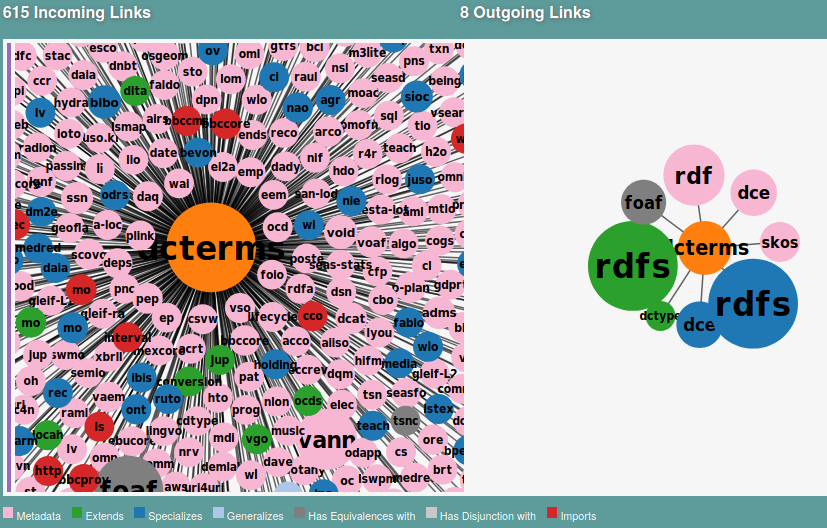
\includegraphics[width=13cm]{images/onto_dcterms.png}
	\caption[L'ontologie DC Terms]{DC Terms: représentation des ontologies l'utilisant (à gauche) et de celles qu'elle utilise(à droite) [Source: \url{https://lov.linkeddata.es/dataset/lov/vocabs/dcterms}]}
	\label{onto_dcterms}
\end{figure}
\medskip

Les \index[ref]{typologie@Typologie!ontologie@Ontologie}ontologies propres aux institutions patrimoniales utilisent ces ontologies de haut niveau. Ainsi, \index[ref]{modelisation@Modélisation!bibo@bibo}\ac{bibo} utilise à la fois les \index[ref]{relier@Relier!dcterms@DC Terms}DC Terms et \index[ref]{relier@Relier!foaf@FOAF}\ac{foaf}. \index[ref]{modelisation@Modélisation!cidoc@CIDOC-CRM}\ac{cidoccrm}\footnote{Voir \reference{annexe_onto} (\reference{onto_c4o})}, contrairement aux autres ontologies institutionnelles, n'est pas de bas niveau, mais de haut niveau. En effet, elle souhaite pouvoir décrire n'importe quel type d'objet: elle dispose de quatre-vingt-cinq classes et de plus de deux cent cinquante propriétés.